\documentclass[9pt,twocolumn,twoside]{gsajnl}
\articletype{inv} % article type
\usepackage{hyperref}
\newcommand{\X}{\textcolor{red}{\bf X\,}}
\newcommand{\citex}{\textcolor{red}{\bf (CITE)\,}}
\newcommand{\jri}[1]{\textcolor{red}{ \emph{ #1}} }
\newcommand{\kc}[1]{\textcolor{blue}{ \emph{ #1}} }

\title{The dynamics of selection and adaptive diversity in modern maize inbred lines}

\author[$\ast$,1]{Kate Crosby}
\author[$\S$]{Justin Gerke}
\author[$\dagger$]{Oscar ``Howie'' Smith}
\author[$\ddagger$,1]{Jeffrey Ross-Ibarra}
%\author[$\ast\ast$]{Author Five}

\affil[$\ast$]{Author one affiliation}
\affil[$\S$]{Author two affiliation}
\affil[$\dagger$]{Author three affiliation}
\affil[$\ddagger$]{Author four affiliation}
%\affil[$\ast\ast$]{Author five affiliation}

\keywords{maize; inbreds; selection; adaptive diversity}

\runningtitle{Modern maize adaptive diversity} % For use in the footer 

\correspondingauthor{Corresponding Author}

\begin{abstract}

blah blah

\end{abstract}

\setboolean{displaycopyright}{true}

\begin{document}

\maketitle
\thispagestyle{firststyle}
\marginmark
\firstpagefootnote
\correspondingauthoraffiliation{Please insert the affiliation correspondence address and email for the corresponding author. The corresponding author should be marked with a `1' in the author list, as shown in the example.}
\vspace{-11pt}%


%For the authors' names, indicate different affiliations with the symbols: $\ast$,  $\S$, $\dagger$, $\ddagger$. After four authors, the symbols double, triple, quadruple, and so forth as required.


\section*{Introduction}

\lettrine[lines=2]{\color{color2}M}{}aize is a staple crop in the United States making up 80 million acres and producing X weight in animal feed. 
Maize yields (a fitness proxy) in the United States have increased in terms of total numbers since the late 1800s, but have largely slowed in terms of growth rate since the influx of new adaptive material in the mid 1950s to early 1970s. As growth rate in fitness is generally correlated with the amount of available adaptive genetic diversity 
Total decrease in heterozygosity amongst and within heterotic breeding pools (cite Gerke - maybe give more of an example here) of modern maize, suggests that genetic diversity is lower than it once was. 
If much of the diversity that has been lost is adaptive, then present day lines would have less variation available to respond to various selection regimes imposed by breeders. 
If diversity has indeed been lost over time, and has not been recouped by the introgression of new material or mutational input, then what is the composition of this lost genetic diversity? Previous studies suggest that \kc{find lit. on this}...
\jri{note in gerke paper that haplotypes fixed (presumably under selection) not found in lines derived from those cycles, suggesting perhaps that adaptive haps have been lost.}
If the loss is largely composed of deleterious or neutral alleles, then the loss is not of concern to farmers and breeders. 
If this loss contains even a small amount of beneficial/adaptive alleles, this would mean that the efficacy of selection on modern maize lines would suffer as time went on. 
This is because, save for the inputs of novel variation in the 1950s when heterotic breeding pools were originally formed - there has not been much in terms of inputs from novel maize material save for... \kc{cite tropical introgression for blight stuff}.


The "inbred-hybrid" selection method for propagating and distributing maize hybrids has been in use for over 100 years in many breeding platforms and programs in the United States. 
This method typically (but not always) selects on inbred "general combining ability" to produce a vigorous and viable hybrid, which is then sold to and grown by farmers. 
These breeding programs may also apply selective agents (drought, disease) to further evaluate combining ability of inbreds.
The loss of heterosis or "hybrid breakdown" then occurs in the next generation, with a loss in fitness/yield, and farmers obtain new F1 hybrids from new inbred combinations.
Phenotypic selection by breeders using mapping populations was a common practice prior to the advent of molecular markers. 
While past studies have found signatures of selection in modern maize: list (cite,cite,cite) these studies have largely fallen short in finding signatures of selection and the polygenic basis of likely many traits under the influence of selection. 
Large effect quantitative trait loci (QTL) and SNPs at these loci are generally markers that are consistently observed to be associated with traits across or within environments. 
However, the genetic basis of most adaptive traits is likely to be polygenic in nature, with each quantitative trait affected by many alleles of small effect \kc{cite examples Doebley, etc Rockman review, Yeaman et al 2015}. We attempt to apply a new method to isolate this signature of polygenic adaptation to our panel of inbred lines.

We focus narrowly on an inbred line's year release date to pinpoint these signatures of selection through time (compare and contrast with Joost) within a heterotic group or genetic cluster as past studies have failed to account for population structure, which may influence a study's power to detect selection \kc{explain the concept of heterotic group or breeding pool above?}. 



\section*{Materials and Methods}

In order to examine selection through time we obtained the exact release dates of 823 public maize inbred lines, using a variety of sources including: Gerdes and Tracy, the USDA database, original line release sheets, or communication with maize breeding experts. Many dates in the USDA although categorized as "Year Released" are the year that the line was acquired. 
The release date indicates the year that line was released to breeders in order to propagate hybrids.
First we grouped inbred lines according to their broad genetic cluster (or 'heterotic group') using principal components analysis (PCA) using the approach described in  \kc{cite plos one G Abraham} or \textit{flashpca} \kc{give githubrepo}. 
This approach is robust to missing SNP data, and is computationally fast for large datasets.  
Maize inbred lines within a broad heterotic group were then dated by year of release, any inbred line without a year of release affiliated with it was discarded from further analysis.



\subsection*{Statistical Analysis} 
To isolate signals of selection and local adaptation within each genetic cluster of maize inbreds, we used BayEnv2 \citep{Coop:2010ke} to estimate Bayes factors ($\beta$). Bayes factors broadly approximate the parameter $Ns$ (population size and selection coefficient).
We estimated the neutral covariance matrix of a subset of polymorphic GBS markers within each genetic cluster. We chose a multiple of the subset of the total GBS markers by chromosome. 
Given that there was approximately 1 marker/1 Mb \kc{orwhatever} these markers are at the very least not cis-linked, which is key to estimating the covariance matrix \kc{basically I took a medium factor of the total length of each cluster - so every 25th -50th marker, it's not random, that's the point - it minimizes LD}. 
The covariance matrix is used to estimate a neutral (drift) model of evolution across environments, in this case temporal environments. 
Thus, any Bayes Factor for a SNP that deviates substantially from expected neutral frequencies has potentially experienced and responded to selection through time.  While there is no strict significance cut-off, large $\beta$s for many SNPs in the same genomic region indicate past selection.
Each inbred line with a release year within a cluster was effectively treated as a population. 
While the approach of treating individuals as populations is not typical of other example studies using BayEnv, it deals directly with the issue of population structure - by testing each SNP in each inbred line (as if it were a population). 

The second approach scans the genome for signals of polygenic adaptation of quantitative traits. This method termed ``$Q_x$'', is first described in \verb|\citep{berg2014population}| and is a novel, multi-variate approach that extends from the univariate $Q_{ST}$ and $F_{ST}$ tests for divergent selection and adaptation \kc{Latta 1998, reviewed in McKay and Latta 2002}. 
As this approach is relatively new, we describe our approach below.

First, GWAS hits (SNP effect sizes) in a mapping population are used to pinpoint SNPs in the genome that significantly contribute to additive genetic variation $V_A$ in quantitative traits, the frequency of those SNPs that have is calculated in the mapping panel. 
To obtain SNP effect sizes, we performed a custom forward stepwise GWAS for the RILs (recombinant inbred lines) produced from 26 half-sib families from the nested associated mapping (NAM) maize population, which also have GBS 2.7 marker coverage.
We used the chromosome specific residuals of 37 traits from \verb|\citep{Wallace:2014db}| (methods to obtain chromosome specific residuals described therein) to perform this custom GWAS. 
From the NAM RILs, we first dropped all alleles that were not biallelic or contained indels and imputed the data to complete cases \kc{(for X markers)} based on allele frequency for a given SNP \href{https://github.com/RILAB/historical_genomics/blob/master/scripts/bulk_imputation_script1.R}{(script available from github)}. 
SNP data was imputed to completeness in order to facilitate forward stepwise regression (see section further down) and model comparison.  

Using the imputed data, we first performed regression of each SNP (by chromosome) to trait residuals, conservatively adjusted all SNP p-values using Bonnferroni correction, and chose the top 500 SNPs on each chromosome (the SNPs with the lowest p-values). 
Forward stepwise regression was then performed for the 500 SNPs with the lowest p-values (by chromosome) to obtain SNP effect sizes for all 37 traits residuals \href{https://github.com/RILAB/historical_genomics/blob/master/scripts/single_step_NAM_script_2.R}{(stepwise regression script available from github)}. 
The SNPs from each chromosome forward stepwise model were then further filtered by choosing the SNP with the lowest p-value within a 100Mb window \href{https://github.com/RILAB/historical_genomics/blob/master/scripts/filter_snp_effects_script_3.R}{(script to filter SNPs by chromosome available from github)}. 
This set of further filtered SNPs was carried forward and regressed again by chromosome to trait residuals in order to obtain SNP effect sizes \href{https://github.com/RILAB/historical_genomics/blob/master/scripts/final_effects_script_4.R}{(script to index 500 SNPs, pull out by index and regress again available on github)}.
One of the motivations for performing all of these single and stepwise regressions by chromosome as opposed to genome wide was to minimize the effect of large clusters of SNPs of significant effect (or large QTL) on a given chromosome, as the overall goal of this method is to isolate even the smallest signals of polygenic adaptation.

Second, using our test population (the Ames panel), the frequencies of those matching SNPs are also calculated. 
Neutral evolution, like in BayEnv is modelled using a covariance matrix of randomly sampled markers to build a multivariate distribution (simulating the genomic background), and this is generally how the method differs from $Q_{ST}$-$F_{ST}$ approaches.
If those SNPs with large effect sizes are at higher frequency in the reference panel than what is expected under the multivariate distribution (the genomic background), then we conclude that there is a signal of polygenic adaptation for the phenotypic trait of interest.
In the univariate scenario (for a given quantitative trait), divergent selection or local adaptation are processes that typically lead to $Q_{ST}$ values > $F_{ST}$ values for both neutral markers and QTLs.
$Q_x$ is a statistic produced for each genetic cluster.

 
P-values of populations that do not fall beyond the asymptotic $Q_x$ value are not different from that expected value given GWAS SNP effect sizes and observed allele frequencies given a neutral covariance matrix (simulated from allel

We performed tests within each genetic cluster

Our final approach used a more recent version of \kc{Nielsen} of finding the signature of positive selection using SWeeD

\subsection*{Data Availability}

Data for GBS 2.7 are available on PANZEA.\jri{add linke} All scripts are available on github (give directory).

%At the end of the Materials and Methods section, include a statement on reagent and data availability. Please read the Data and Reagent Policy before writing the statement. Make sure to list the accession numbers or DOIs of any data you have placed in public repositories. List the file names an descriptions of any data you will upload as supplemental information. The statement should also include any applicable IRB numbers. You may include specifications for how to properly acknowledge or cite the data.

%For example: Strains are available upon request. File S1 contains detailed descriptions of all supplemental files. File S2 contains SNP ID numbers and locations. File S3 contains genotypes for each individual. Sequence data are available at GenBank and the accession numbers are listed in File S3. Gene expression data are available at GEO with the accession number: GDS1234. Code used to generate the simulated data is provided in file S4. 


\section*{Results and Discussion}

\subsection{Identification of heterotic groups}
We isolated and identified six genetic cluster from the Ames panel (Fig. 1). Clusters 4 and 6 contained lines with no release years.
\begin{figure}[htbp]
\centering
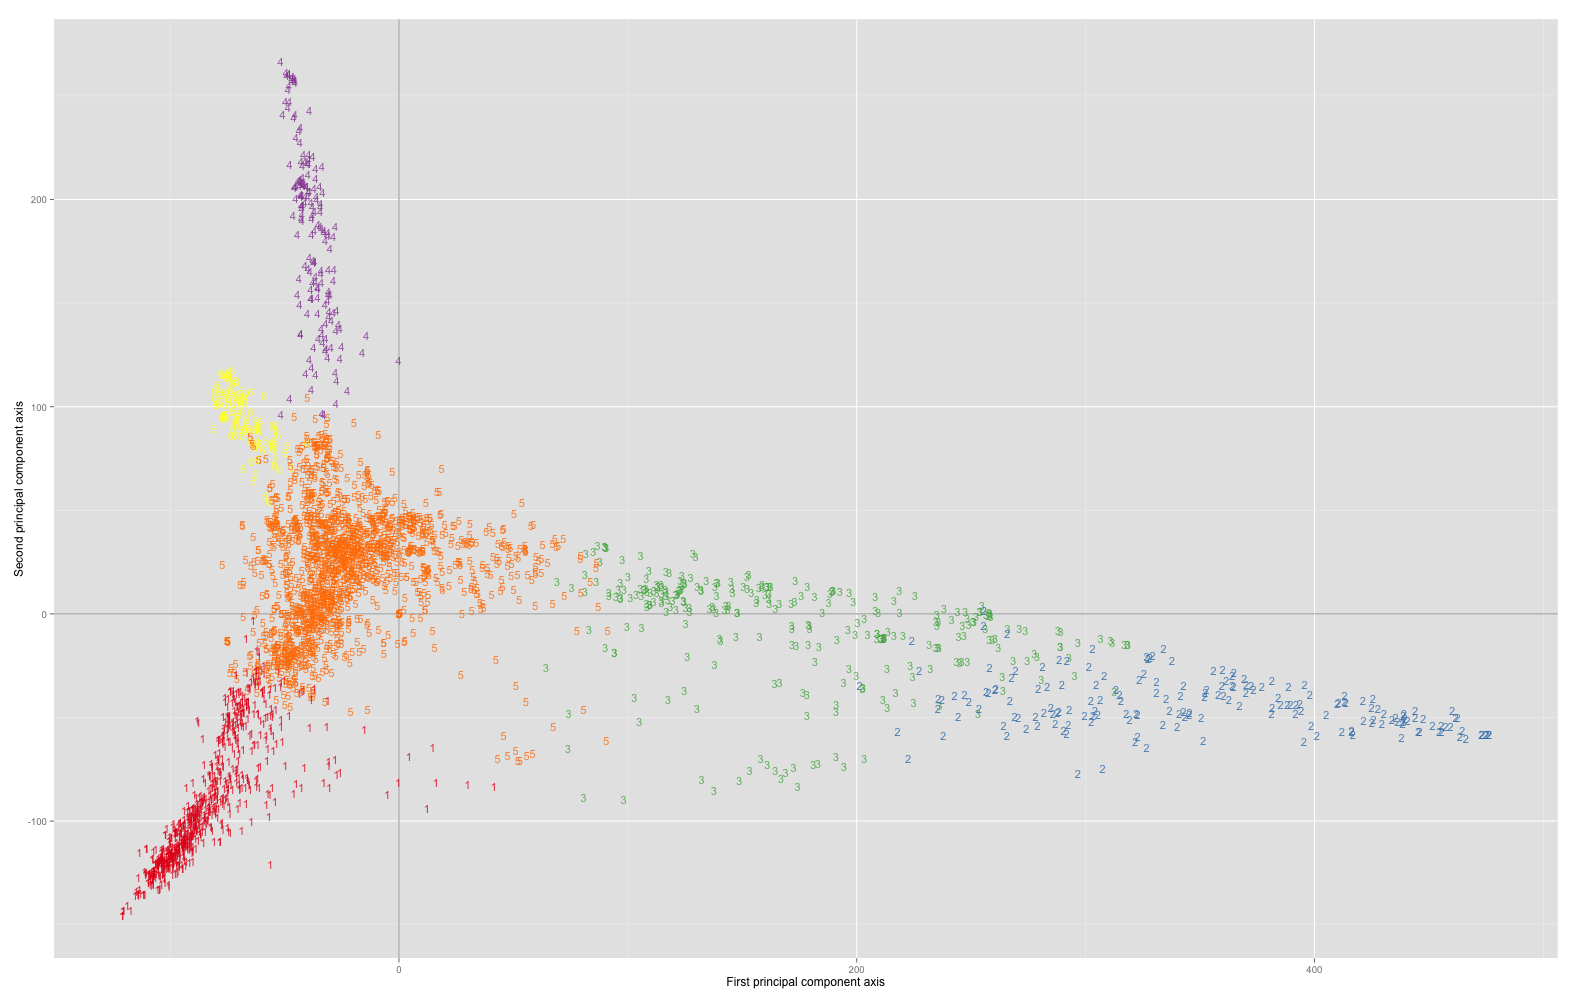
\includegraphics[width=\linewidth]{6_clusters_placeholder.png}
\caption{Six genetic clusters representing the broad heterotic groups of modern maize from the Ames panel using GBS 2.7 aligned to version 3 of the B73 genome 
}
\label{fig:6clusters}
\end{figure}


\begin{figure}[htbp]
\centering
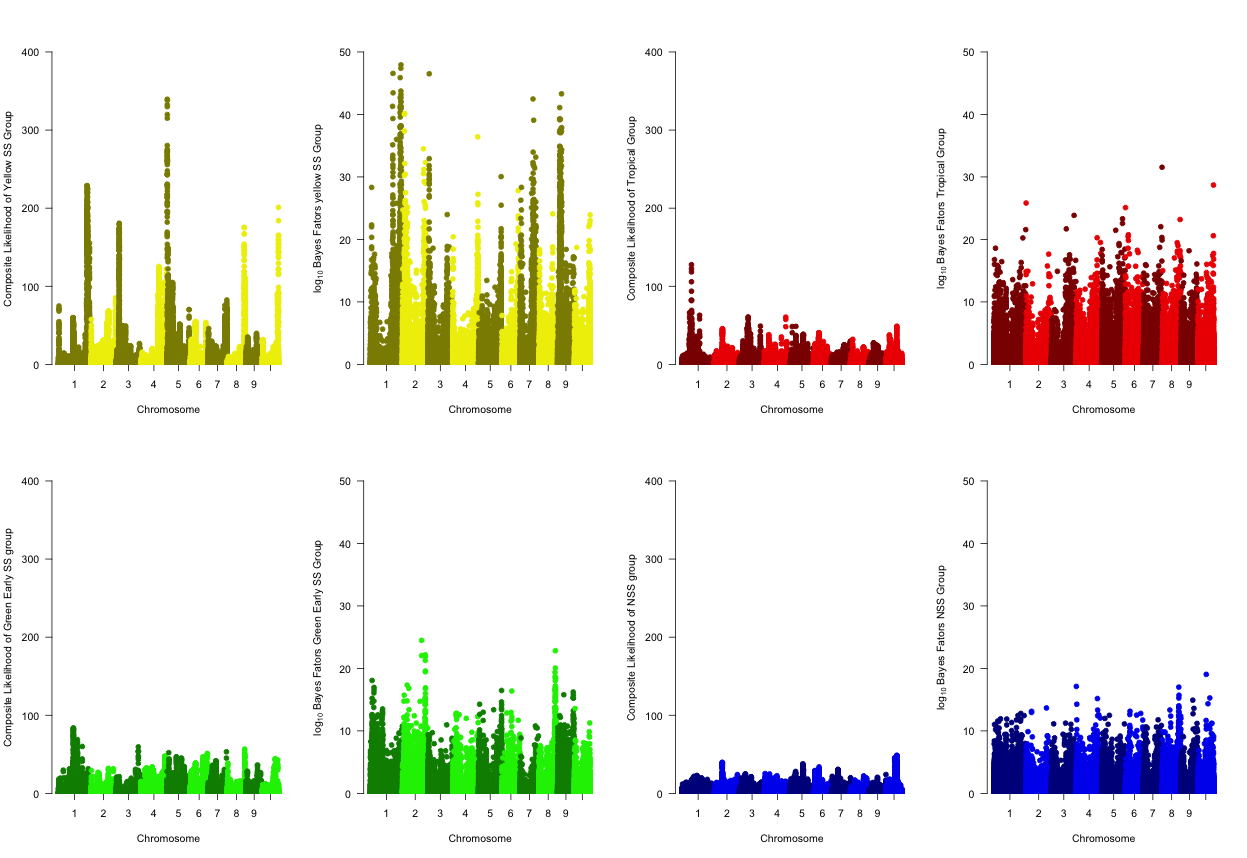
\includegraphics[width=\linewidth]{manhattan_mania.png}
\caption{Manhattan plots of scans of selection with $log_10$ transformed Bayes factors as calculated from Bayenv2 and SweeD for each cluster
}
\label{fig:manhattan}
\end{figure}


\section*{Acknowledgements}
Financial support for this work came from NSF grant IOS-1238014, USDA grant 2009-65300-05668, and DuPont Pioneer.  We'd like to thank DuPont Pioneer as well for their kind support gathering information about years of release. We thank Graham Coop, Jeremy Berg, James Holland, Edward Buckler, \X and \X reviewers for helpful discussion. 

\bibliography{example-bibliography}

\end{document}